

\tikzset{every picture/.style={line width=0.75pt}} %set default line width to 0.75pt        

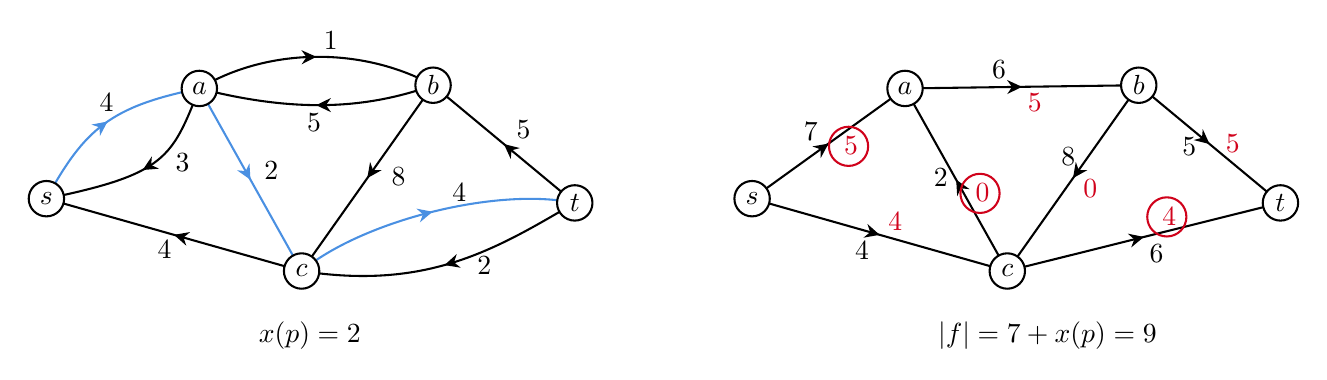
\begin{tikzpicture}[x=0.5pt,y=0.5pt,yscale=-1,xscale=1]
%uncomment if require: \path (0,252); %set diagram left start at 0, and has height of 252

%Curve Lines [id:da5613638706519646] 
\draw [color={rgb, 255:red, 74; green, 144; blue, 226 }  ,draw opacity=1 ]   (202.22,187) .. controls (245.5,151) and (342.5,126) .. (399.62,137.78) ;
\draw [shift={(296.83,144.2)}, rotate = 525.5699999999999] [fill={rgb, 255:red, 74; green, 144; blue, 226 }  ,fill opacity=1 ][line width=0.08]  [draw opacity=0] (10.72,-5.15) -- (0,0) -- (10.72,5.15) -- (7.12,0) -- cycle    ;
%Curve Lines [id:da2735285843771139] 
\draw [color={rgb, 255:red, 74; green, 144; blue, 226 }  ,draw opacity=1 ]   (17.79,134.72) .. controls (45.5,84) and (64.5,68) .. (128.31,55.06) ;
\draw [shift={(61.98,78.96)}, rotate = 503.55] [fill={rgb, 255:red, 74; green, 144; blue, 226 }  ,fill opacity=1 ][line width=0.08]  [draw opacity=0] (10.72,-5.15) -- (0,0) -- (10.72,5.15) -- (7.12,0) -- cycle    ;
%Curve Lines [id:da6525683976596537] 
\draw    (128.31,55.06) .. controls (108.5,105) and (104.5,117) .. (17.79,134.72) ;
\draw [shift={(87.35,114.01)}, rotate = 329.68] [fill={rgb, 255:red, 0; green, 0; blue, 0 }  ][line width=0.08]  [draw opacity=0] (10.72,-5.15) -- (0,0) -- (10.72,5.15) -- (7.12,0) -- cycle    ;
%Curve Lines [id:da9916324740026169] 
\draw    (128.31,55.06) .. controls (176.5,26) and (244.5,24) .. (297.22,52.73) ;
\draw [shift={(212.84,32.2)}, rotate = 538.53] [fill={rgb, 255:red, 0; green, 0; blue, 0 }  ][line width=0.08]  [draw opacity=0] (10.72,-5.15) -- (0,0) -- (10.72,5.15) -- (7.12,0) -- cycle    ;
%Curve Lines [id:da8306124055787136] 
\draw    (297.22,52.73) .. controls (246.5,71) and (194.5,72) .. (128.31,55.06) ;
\draw [shift={(212.74,67.12)}, rotate = 359.78] [fill={rgb, 255:red, 0; green, 0; blue, 0 }  ][line width=0.08]  [draw opacity=0] (10.72,-5.15) -- (0,0) -- (10.72,5.15) -- (7.12,0) -- cycle    ;
%Curve Lines [id:da21823822635678936] 
\draw    (399.62,137.78) .. controls (341.5,172) and (292.5,201) .. (202.22,187) ;
\draw [shift={(305.51,182.7)}, rotate = 343.65] [fill={rgb, 255:red, 0; green, 0; blue, 0 }  ][line width=0.08]  [draw opacity=0] (10.72,-5.15) -- (0,0) -- (10.72,5.15) -- (7.12,0) -- cycle    ;
%Straight Lines [id:da06700183790814418] 
\draw    (202.22,187) -- (297.22,52.73) ;
\draw [shift={(249.72,119.86)}, rotate = 305.28] [fill={rgb, 255:red, 0; green, 0; blue, 0 }  ][line width=0.08]  [draw opacity=0] (10.72,-5.15) -- (0,0) -- (10.72,5.15) -- (7.12,0) -- cycle    ;
%Straight Lines [id:da78660649581525] 
\draw [color={rgb, 255:red, 74; green, 144; blue, 226 }  ,draw opacity=1 ]   (128.31,55.06) -- (202.22,187) ;
\draw [shift={(165.27,121.03)}, rotate = 240.74] [fill={rgb, 255:red, 74; green, 144; blue, 226 }  ,fill opacity=1 ][line width=0.08]  [draw opacity=0] (10.72,-5.15) -- (0,0) -- (10.72,5.15) -- (7.12,0) -- cycle    ;
%Straight Lines [id:da8749205218684325] 
\draw    (202.22,187) -- (17.79,134.72) ;
\draw [shift={(110.01,160.86)}, rotate = 375.83000000000004] [fill={rgb, 255:red, 0; green, 0; blue, 0 }  ][line width=0.08]  [draw opacity=0] (10.72,-5.15) -- (0,0) -- (10.72,5.15) -- (7.12,0) -- cycle    ;
%Straight Lines [id:da4360222788208358] 
\draw    (297.22,52.73) -- (399.62,137.78) ;
\draw [shift={(348.42,95.26)}, rotate = 39.71] [fill={rgb, 255:red, 0; green, 0; blue, 0 }  ][line width=0.08]  [draw opacity=0] (10.72,-5.15) -- (0,0) -- (10.72,5.15) -- (7.12,0) -- cycle    ;
%Shape: Ellipse [id:dp22199319065994672] 
\draw  [fill={rgb, 255:red, 255; green, 255; blue, 255 }  ,fill opacity=1 ] (5,134.72) .. controls (5,127.66) and (10.73,121.93) .. (17.79,121.93) .. controls (24.86,121.93) and (30.58,127.66) .. (30.58,134.72) .. controls (30.58,141.78) and (24.86,147.51) .. (17.79,147.51) .. controls (10.73,147.51) and (5,141.78) .. (5,134.72) -- cycle ;
%Shape: Ellipse [id:dp734016786907147] 
\draw  [fill={rgb, 255:red, 255; green, 255; blue, 255 }  ,fill opacity=1 ] (115.52,55.06) .. controls (115.52,48) and (121.25,42.27) .. (128.31,42.27) .. controls (135.38,42.27) and (141.1,48) .. (141.1,55.06) .. controls (141.1,62.13) and (135.38,67.85) .. (128.31,67.85) .. controls (121.25,67.85) and (115.52,62.13) .. (115.52,55.06) -- cycle ;
%Shape: Ellipse [id:dp6263378369405302] 
\draw  [fill={rgb, 255:red, 255; green, 255; blue, 255 }  ,fill opacity=1 ] (284.43,52.73) .. controls (284.43,45.66) and (290.15,39.94) .. (297.22,39.94) .. controls (304.28,39.94) and (310.01,45.66) .. (310.01,52.73) .. controls (310.01,59.79) and (304.28,65.52) .. (297.22,65.52) .. controls (290.15,65.52) and (284.43,59.79) .. (284.43,52.73) -- cycle ;
%Shape: Ellipse [id:dp7990256965184968] 
\draw  [fill={rgb, 255:red, 255; green, 255; blue, 255 }  ,fill opacity=1 ] (189.43,187) .. controls (189.43,179.94) and (195.15,174.21) .. (202.22,174.21) .. controls (209.28,174.21) and (215.01,179.94) .. (215.01,187) .. controls (215.01,194.06) and (209.28,199.79) .. (202.22,199.79) .. controls (195.15,199.79) and (189.43,194.06) .. (189.43,187) -- cycle ;
%Shape: Ellipse [id:dp7073963568621764] 
\draw  [fill={rgb, 255:red, 255; green, 255; blue, 255 }  ,fill opacity=1 ] (386.83,137.78) .. controls (386.83,130.72) and (392.56,124.99) .. (399.62,124.99) .. controls (406.69,124.99) and (412.41,130.72) .. (412.41,137.78) .. controls (412.41,144.85) and (406.69,150.57) .. (399.62,150.57) .. controls (392.56,150.57) and (386.83,144.85) .. (386.83,137.78) -- cycle ;
%Straight Lines [id:da5195310081734267] 
\draw    (712.22,187) -- (807.22,52.73) ;
\draw [shift={(759.72,119.86)}, rotate = 305.28] [fill={rgb, 255:red, 0; green, 0; blue, 0 }  ][line width=0.08]  [draw opacity=0] (10.72,-5.15) -- (0,0) -- (10.72,5.15) -- (7.12,0) -- cycle    ;
%Straight Lines [id:da4538291997735936] 
\draw    (638.31,55.06) -- (712.22,187) ;
\draw [shift={(675.27,121.03)}, rotate = 60.74] [fill={rgb, 255:red, 0; green, 0; blue, 0 }  ][line width=0.08]  [draw opacity=0] (10.72,-5.15) -- (0,0) -- (10.72,5.15) -- (7.12,0) -- cycle    ;
%Straight Lines [id:da7538382565478482] 
\draw    (527.79,134.72) -- (712.22,187) ;
\draw [shift={(620.01,160.86)}, rotate = 195.83] [fill={rgb, 255:red, 0; green, 0; blue, 0 }  ][line width=0.08]  [draw opacity=0] (10.72,-5.15) -- (0,0) -- (10.72,5.15) -- (7.12,0) -- cycle    ;
%Straight Lines [id:da6748069532380702] 
\draw    (909.62,137.78) -- (712.22,187) ;
\draw [shift={(810.92,162.39)}, rotate = 166] [fill={rgb, 255:red, 0; green, 0; blue, 0 }  ][line width=0.08]  [draw opacity=0] (10.72,-5.15) -- (0,0) -- (10.72,5.15) -- (7.12,0) -- cycle    ;
%Straight Lines [id:da3976427132067899] 
\draw    (527.79,134.72) -- (638.31,55.06) ;
\draw [shift={(583.05,94.89)}, rotate = 504.22] [fill={rgb, 255:red, 0; green, 0; blue, 0 }  ][line width=0.08]  [draw opacity=0] (10.72,-5.15) -- (0,0) -- (10.72,5.15) -- (7.12,0) -- cycle    ;
%Straight Lines [id:da5989756628707282] 
\draw    (807.22,52.73) -- (909.62,137.78) ;
\draw [shift={(858.42,95.26)}, rotate = 219.71] [fill={rgb, 255:red, 0; green, 0; blue, 0 }  ][line width=0.08]  [draw opacity=0] (10.72,-5.15) -- (0,0) -- (10.72,5.15) -- (7.12,0) -- cycle    ;
%Straight Lines [id:da8582315780180115] 
\draw    (638.31,55.06) -- (807.22,52.73) ;
\draw [shift={(722.76,53.89)}, rotate = 539.21] [fill={rgb, 255:red, 0; green, 0; blue, 0 }  ][line width=0.08]  [draw opacity=0] (10.72,-5.15) -- (0,0) -- (10.72,5.15) -- (7.12,0) -- cycle    ;
%Shape: Ellipse [id:dp48011285603633225] 
\draw  [fill={rgb, 255:red, 255; green, 255; blue, 255 }  ,fill opacity=1 ] (515,134.72) .. controls (515,127.66) and (520.73,121.93) .. (527.79,121.93) .. controls (534.86,121.93) and (540.58,127.66) .. (540.58,134.72) .. controls (540.58,141.78) and (534.86,147.51) .. (527.79,147.51) .. controls (520.73,147.51) and (515,141.78) .. (515,134.72) -- cycle ;
%Shape: Ellipse [id:dp34527564053657145] 
\draw  [fill={rgb, 255:red, 255; green, 255; blue, 255 }  ,fill opacity=1 ] (625.52,55.06) .. controls (625.52,48) and (631.25,42.27) .. (638.31,42.27) .. controls (645.38,42.27) and (651.1,48) .. (651.1,55.06) .. controls (651.1,62.13) and (645.38,67.85) .. (638.31,67.85) .. controls (631.25,67.85) and (625.52,62.13) .. (625.52,55.06) -- cycle ;
%Shape: Ellipse [id:dp6239749822676505] 
\draw  [fill={rgb, 255:red, 255; green, 255; blue, 255 }  ,fill opacity=1 ] (794.43,52.73) .. controls (794.43,45.66) and (800.15,39.94) .. (807.22,39.94) .. controls (814.28,39.94) and (820.01,45.66) .. (820.01,52.73) .. controls (820.01,59.79) and (814.28,65.52) .. (807.22,65.52) .. controls (800.15,65.52) and (794.43,59.79) .. (794.43,52.73) -- cycle ;
%Shape: Ellipse [id:dp4869792682336288] 
\draw  [fill={rgb, 255:red, 255; green, 255; blue, 255 }  ,fill opacity=1 ] (699.43,187) .. controls (699.43,179.94) and (705.15,174.21) .. (712.22,174.21) .. controls (719.28,174.21) and (725.01,179.94) .. (725.01,187) .. controls (725.01,194.06) and (719.28,199.79) .. (712.22,199.79) .. controls (705.15,199.79) and (699.43,194.06) .. (699.43,187) -- cycle ;
%Shape: Ellipse [id:dp8101897126294262] 
\draw  [fill={rgb, 255:red, 255; green, 255; blue, 255 }  ,fill opacity=1 ] (896.83,137.78) .. controls (896.83,130.72) and (902.56,124.99) .. (909.62,124.99) .. controls (916.69,124.99) and (922.41,130.72) .. (922.41,137.78) .. controls (922.41,144.85) and (916.69,150.57) .. (909.62,150.57) .. controls (902.56,150.57) and (896.83,144.85) .. (896.83,137.78) -- cycle ;

% Text Node
\draw (527.79,134.72) node   [align=left] {$\displaystyle s$};
% Text Node
\draw (638.31,55.06) node   [align=left] {$\displaystyle a$};
% Text Node
\draw (807.22,52.73) node   [align=left] {$\displaystyle b$};
% Text Node
\draw (712.22,187) node   [align=left] {$\displaystyle c$};
% Text Node
\draw (909.62,137.78) node   [align=left] {$\displaystyle t$};
% Text Node
\draw (600,163.89) node [anchor=north west][inner sep=0.75pt]   [align=left] {$\displaystyle 4$};
% Text Node
\draw (749,95.89) node [anchor=north west][inner sep=0.75pt]   [align=left] {$\displaystyle 8$};
% Text Node
\draw (657,110.89) node [anchor=north west][inner sep=0.75pt]   [align=left] {$\displaystyle 2$};
% Text Node
\draw (563,77.89) node [anchor=north west][inner sep=0.75pt]   [align=left] {$\displaystyle 7$};
% Text Node
\draw (812.92,165.39) node [anchor=north west][inner sep=0.75pt]   [align=left] {$\displaystyle 6$};
% Text Node
\draw (836.42,88.26) node [anchor=north west][inner sep=0.75pt]   [align=left] {$\displaystyle 5$};
% Text Node
\draw (699,32.89) node [anchor=north west][inner sep=0.75pt]   [align=left] {$\displaystyle 6$};
% Text Node
\draw (624,142.89) node [anchor=north west][inner sep=0.75pt]   [align=left] {$\displaystyle \textcolor[rgb]{0.82,0.01,0.11}{4}$};
% Text Node
\draw  [color={rgb, 255:red, 208; green, 2; blue, 27 }  ,draw opacity=1 ]  (692.5, 130.89) circle [x radius= 14.15, y radius= 14.15]   ;
\draw (687,121.89) node [anchor=north west][inner sep=0.75pt]   [align=left] {$\displaystyle \textcolor[rgb]{0.82,0.01,0.11}{0}$};
% Text Node
\draw  [color={rgb, 255:red, 208; green, 2; blue, 27 }  ,draw opacity=1 ]  (827.5, 147.89) circle [x radius= 14.15, y radius= 14.15]   ;
\draw (822,138.89) node [anchor=north west][inner sep=0.75pt]   [align=left] {$\displaystyle \textcolor[rgb]{0.82,0.01,0.11}{4}$};
% Text Node
\draw  [color={rgb, 255:red, 208; green, 2; blue, 27 }  ,draw opacity=1 ]  (597.5, 96.89) circle [x radius= 14.15, y radius= 14.15]   ;
\draw (592,87.89) node [anchor=north west][inner sep=0.75pt]   [align=left] {$\displaystyle \textcolor[rgb]{0.82,0.01,0.11}{5}$};
% Text Node
\draw (724.76,56.89) node [anchor=north west][inner sep=0.75pt]   [align=left] {$\displaystyle \textcolor[rgb]{0.82,0.01,0.11}{5}$};
% Text Node
\draw (765,118.89) node [anchor=north west][inner sep=0.75pt]   [align=left] {$\displaystyle \textcolor[rgb]{0.82,0.01,0.11}{0}$};
% Text Node
\draw (868,85.89) node [anchor=north west][inner sep=0.75pt]   [align=left] {$\displaystyle \textcolor[rgb]{0.82,0.01,0.11}{5}$};
% Text Node
\draw (17.79,134.72) node   [align=left] {$\displaystyle s$};
% Text Node
\draw (128.31,55.06) node   [align=left] {$\displaystyle a$};
% Text Node
\draw (297.22,52.73) node   [align=left] {$\displaystyle b$};
% Text Node
\draw (202.22,187) node   [align=left] {$\displaystyle c$};
% Text Node
\draw (399.62,137.78) node   [align=left] {$\displaystyle t$};
% Text Node
\draw (109,99.89) node [anchor=north west][inner sep=0.75pt]   [align=left] {$\displaystyle 3$};
% Text Node
\draw (265,109.89) node [anchor=north west][inner sep=0.75pt]   [align=left] {$\displaystyle 8$};
% Text Node
\draw (173,105.89) node [anchor=north west][inner sep=0.75pt]   [align=left] {$\displaystyle 2$};
% Text Node
\draw (54,56.89) node [anchor=north west][inner sep=0.75pt]   [align=left] {$\displaystyle 4$};
% Text Node
\draw (308.92,121.39) node [anchor=north west][inner sep=0.75pt]   [align=left] {$\displaystyle 4$};
% Text Node
\draw (355.42,76.26) node [anchor=north west][inner sep=0.75pt]   [align=left] {$\displaystyle 5$};
% Text Node
\draw (216,11.89) node [anchor=north west][inner sep=0.75pt]   [align=left] {$\displaystyle 1$};
% Text Node
\draw (96,162.89) node [anchor=north west][inner sep=0.75pt]   [align=left] {$\displaystyle 4$};
% Text Node
\draw (204,70.89) node [anchor=north west][inner sep=0.75pt]   [align=left] {$\displaystyle 5$};
% Text Node
\draw (326.92,174.39) node [anchor=north west][inner sep=0.75pt]   [align=left] {$\displaystyle 2$};
% Text Node
\draw (169,221.5) node [anchor=north west][inner sep=0.75pt]   [align=left] {$\displaystyle x( p) =2$};
% Text Node
\draw (660,221.5) node [anchor=north west][inner sep=0.75pt]   [align=left] {$\displaystyle |f|=7+x( p) =9$};


\end{tikzpicture}

